% Settings for the default beamer theme
\documentclass[english, aspectratio=169]{beamer}
\usepackage[T1]{fontenc}
\usepackage[utf8]{inputenc}
\usepackage{tabularx}
\usepackage{babel}
\usepackage[ruled,vlined]{algorithm2e}
\SetAlgorithmName{Algoritmus}{algoritmus}{List of Algorithms}
\setcounter{secnumdepth}{3}
\setcounter{tocdepth}{3}

\makeatletter

\newcommand\makebeamertitle{\frame{\maketitle}}

% (ERT) argument for the TOC
\AtBeginDocument{%
  \let\origtableofcontents=\tableofcontents
  \def\tableofcontents{\@ifnextchar[{\origtableofcontents}{\gobbletableofcontents}}
  \def\gobbletableofcontents#1{\origtableofcontents}
}

% Theme settings
\usetheme{Frankfurt}
\usecolortheme{default}
\usefonttheme[onlymath]{serif}

% Template settings
\setbeamertemplate{navigation symbols}{}
\setbeamertemplate{blocks}[rounded][shadow=false]
\setbeamertemplate{title page}[default][colsep=-4bp, rounded=true, shadow=false]
\makeatother

\begin{document}

% Title page
\section{Bevezetés}
\title[]{Üzleti Intelligencia}
\subtitle{6. Előadás: Mély $Q$-tanulási architektúrák}
\author[Kuknyó Dániel]{Kuknyó Dániel\\Budapesti Gazdasági Egyetem}
\date{2023/24\\1.félév}
\makebeamertitle

% Table of contents slide
\begin{frame}
\tableofcontents{}
\end{frame}

% Table of contents of the current section
\begin{frame}
\tableofcontents[currentsection]
\end{frame}

\begin{frame}{A $Q$-tanulás alapjai}
\begin{columns}
\begin{column}{.75\textwidth}
A megerősítéses tanulásban az egyik nagy áttörést egy politikafüggetlen TD algoritmus kifejlesztése hozta el.\par\smallskip
Ebben az esetben a becsült \textbf{állapot-cselekvés minőség függvény}, $Q$, ami megadja, hogy mennyire jövedelmező az ügynöknek $s$ állapotban $a$ cselekvést végrehajtani.
\begin{block}{$Q$-tanulás}
\[
Q(s_t,a_t) \leftarrow Q(s_t,a_t) + \alpha \left[ r_{t+1} + \gamma \underset{a}{max}Q(s_{t+1},a) - Q(s_t,a_t) \right]
\]
\end{block}
A $Q$-tanulás ezáltal egy teljesen online tanulási algoritmus, ami a követett \textbf{politikától függetlenül} garantáltan konvergálni fog a valós $Q$ értékekhez.
\end{column}
\begin{column}{.25\textwidth}
\begin{center}
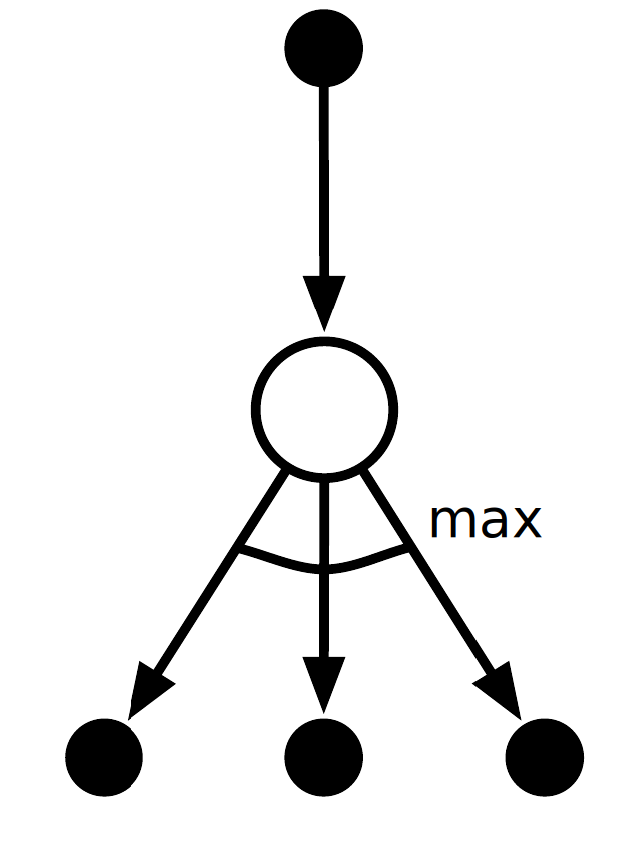
\includegraphics[width=3cm, keepaspectratio]{../../5_ql/doc/images/ql_2.png}
\end{center}
\end{column}
\end{columns}
\end{frame}

\begin{frame}{Dupla $Q$-tanulás}
A kettős tanulás ötlete természetesen kiterjed a teljes MDP algoritmusaira. A $Q$-tanulásban a becsült $Q$-értékek torzítottak lehetnek, ha alacsony a minta számossága, vagy zaj van a rendszerben. Egy módja a $Q$-tanulás regularizálásának, ha egy helyet\textbf{ két $Q$-táblát tart nyilván az algoritmus}, $Q_1$-et és $Q_2$-t.\par\smallskip
A $Q$-tanulással analóg dupla $Q$-tanulás nevű kettős tanulási algoritmus két részre osztja az időlépéseket, \textbf{minden lépésnél egy érmét feldobva}. Ha az érme fejre esik, a frissítés a következő:
\begin{block}{}
\vspace{-0.5cm}
\[
Q_1(s_t,a_t) \leftarrow Q_1(s_t,a_t) + \alpha \left[ r_{t+1} + \gamma Q_2(s_t+1, \underset{a}{argmax} Q_1(s_{t+1},a)) - Q_1(s_t, a_t) \right]
\]
\end{block}
Ha az érme pedig írásra esik, akkor ugyanez a frissítés $Q_1$ és $Q_2$ felcserélésével történik, így $Q_2$ frissül. A két közelítő értékfüggvényt teljesen szimmetrikusan kezeli az algoritmus. Például egy $\varepsilon$-mohó politika a dupla tanulás esetében az egyes cselekvési értékbecslések \textbf{átlagára vagy összegére épülhet}.
\end{frame}

\begin{frame}{Alapvető $Q$-tanulási eljárások}
\begin{columns}
\begin{column}{.5\textwidth}
\begin{center}
$Q$-tanulás\par\smallskip
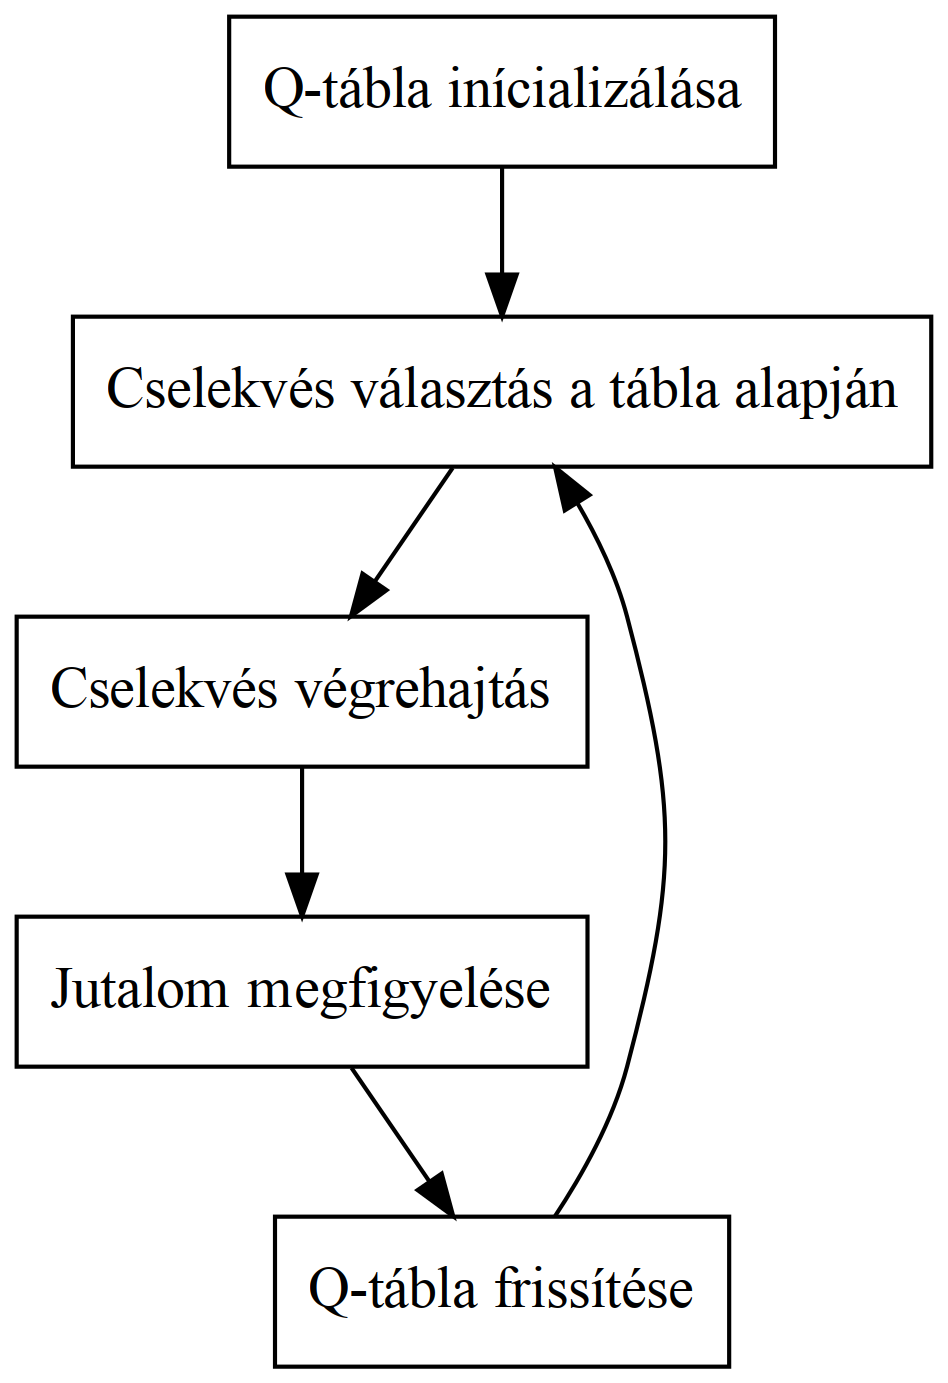
\includegraphics[height=6cm, keepaspectratio]{../../5_ql/doc/graphs/ql_1.png}
\end{center}
\end{column}
\begin{column}{.5\textwidth}
\begin{center}
Dupla $Q$-tanulás\par\smallskip
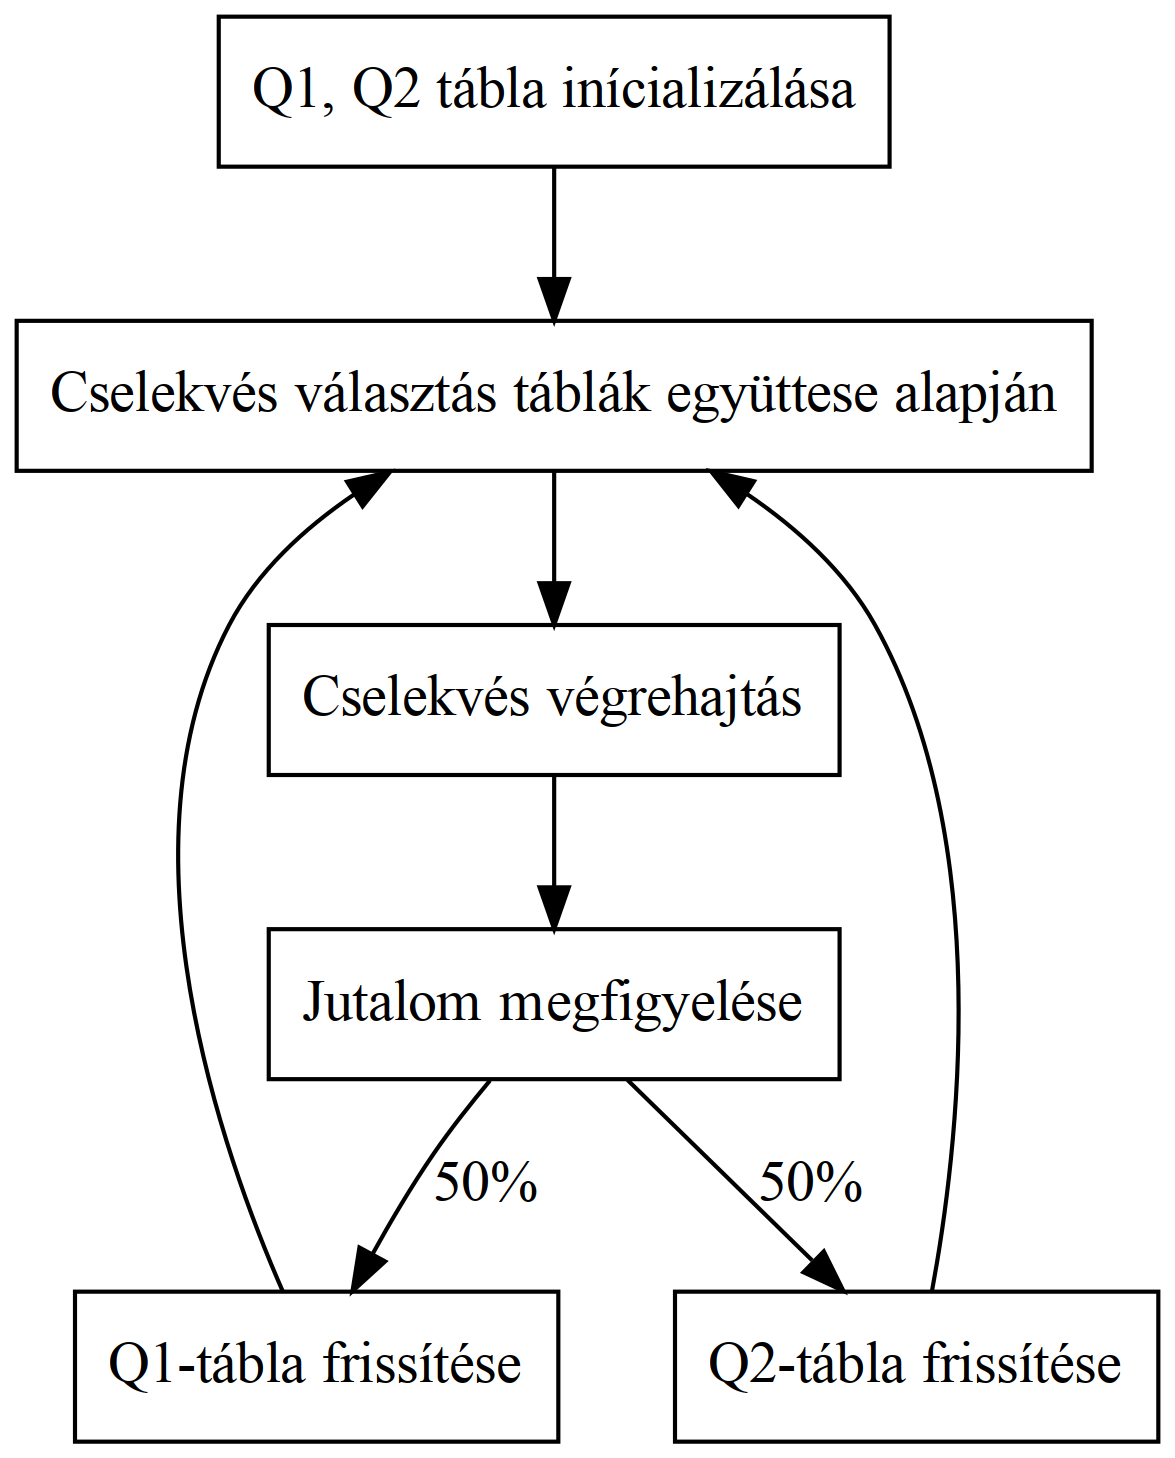
\includegraphics[height=6cm, keepaspectratio]{../../5_ql/doc/graphs/ql_2.png}
\end{center}
\end{column}
\end{columns}
\end{frame}

\section{Mély $Q$-tanulás}

\begin{frame}
\tableofcontents[currentsection]
\end{frame}

\begin{frame}{A $Q$-hálózat (DQN)}
\begin{columns}
\begin{column}{.6\textwidth}
A $Q$-hálózat egy természetes kiterjesztése a hagyományos $Q$-tanulásnak. A naív $Q$-hálózat inputja a \textbf{környezetet leíró változók} vektora vagy mátrixa, és az outputja pedig az ügynök számára elérhető \textbf{cselekvések $Q(s,a)$ értéke} minden $a_1,a_2,..,a_n$ cselekvéshez tartozóan. \par\smallskip
A cselekvés választáshoz az ügynök kiválasztja a \textbf{legnagyobb becsült $Q$ értéket}, és az ahhoz tartozó cselekvést fogja végrehajtani.\par\smallskip
A $Q$-hálózat költségfüggvénye az \textbf{átlagos négyzetes Bellman hiba}, a paraméter frissítése pedig a költségfüggvény gradiense és a lépésméret szerint történik. 
\end{column}
\begin{column}{.4\textwidth}
\begin{center}
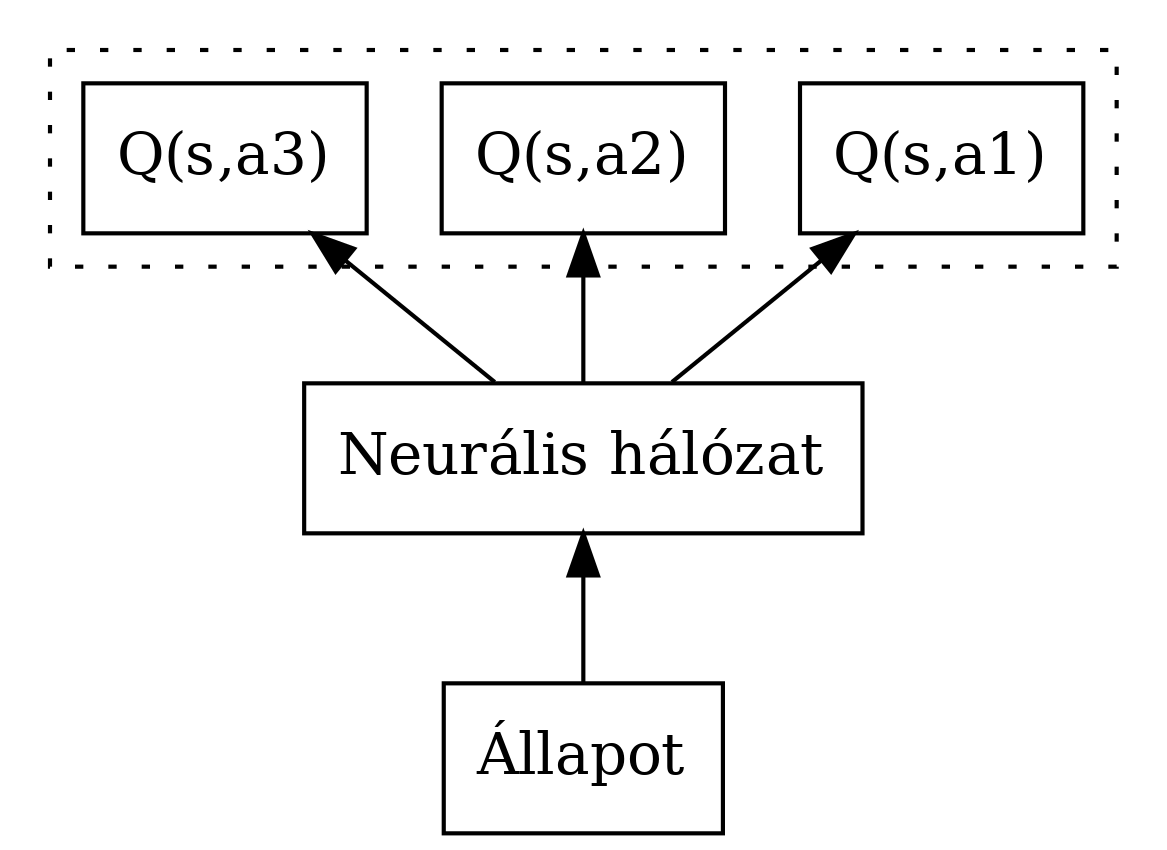
\includegraphics[width=6cm, keepaspectratio]{../../5_ql/doc/graphs/ql_3.png}
\end{center}
\end{column}
\end{columns}
\end{frame}

\begin{frame}{A DQN költségfüggvénye}
\begin{columns}
\begin{column}{.5\textwidth}

\end{column}
\begin{column}{.5\textwidth}
%TODO: insert image
\end{column}
\end{columns}
\end{frame}

\end{document}











